\documentclass[12pt,a4paper]{article}
\usepackage{hw}
\usepackage{tikz}
\usetikzlibrary{arrows}


\graphicspath{ {.} }

\begin{document}
    \qtitle{Q6.8}
    \textbf{a.}\\
    $\mathbf{H}=\newvec{7&0&-3\\-9&-2&3\\18&0&-8}\stackrel{r_3=2r_2+r_3}{\stackrel{r_2=r_1+r_2}{\stackrel{r_1=r_1+3r_2-1.5r_3}{\longeq{6}}}}\newvec{1&0&0\\-2&-2&0\\0&-4&-2}$

    $\newdet{\mathbf{H}-\lambda \mathbf{I}}=0 \Longrightarrow \\
    \newdet{1-\lambda&0&0\\-2&-2-\lambda&0\\0&-4&-2-\lambda}=(1-\lambda)(2+\lambda)^2=0$

    \noindent So the eigenvalues are $\lambda_1=1,\lambda_2=\lambda_3=-2$

    \noindent Then to find eigenvectors, \\
    (1). For $\lambda_1=1$,\\
    $\newvec{6&0&-3\\-9&-3&3\\18&0&-9}*\newvec{u_1\\u_2\\u3}=0\Longrightarrow 6u_1-u_3=0\quad and \quad -9u_1-u_2+u_3=0\\
    u_3=r;\ u_1=0.5r;\ u2=-0.5r \Rightarrow \mathbf{u}=r\newvec{0.5\\-0.5\\1}\Rightarrow \cfrac{1}{\sqrt{6}}\newvec{1\\-1\\2}$

    \noindent (2). For $\lambda_2=\lambda_3=-2$,\\
    $\newvec{9&0&-3\\-9&0&3\\18&0&-6}*\newvec{u_1\\u_2\\u_3}=0\Longrightarrow 3u_1-3u_3=0$\\
    \textbf{I.} when $u_1=u_3=0$, then $u_2=s$, $\mathbf{u}=s\newvec{0\\1\\0}\Rightarrow\newvec{0\\1\\0}$\\
    \textbf{II.} when $u_2=0$, then $u_1=t;\ u_3=3t$, $\mathbf{u}=t\newvec{1\\0\\3}\Rightarrow\cfrac{1}{\sqrt{10}}\newvec{1\\0\\3}$.

    Therefore, eigenvalues are $\mathbf{\Lambda}=\newvec{1&&\\&-2&\\&&-2}$ and eigenvectors are $\mathbf{U}=\newvec{\frac{1}{\sqrt{6}}&0&\frac{1}{\sqrt{10}}\\-\frac{1}{\sqrt{6}}&1&0\\\frac{2}{\sqrt{6}}&0&\frac{3}{\sqrt{10}}}$

    \textbf{b.}\\
     For $\mathbf{H}$, since it's full rank, so $\mathbf{H=U\Lambda U^{-1}}$. If $\mathbf{U}$ is unitary, then $\mathbf{U}^\dagger = \mathbf{U}^{-1}$. That means $\mathbf{H=U\Lambda U^\dagger}$.
     
     $\mathbf{U\Lambda U^\dagger}=\newvec{\cfrac{1}{\sqrt{6}}&0&\cfrac{1}{\sqrt{10}}\\-\cfrac{1}{\sqrt{6}}&1&0\\\cfrac{2}{\sqrt{6}}&0&\cfrac{3}{\sqrt{10}}}\newvec{1&&\\&-2&\\&&-2}\newvec{\cfrac{1}{\sqrt{6}}&-\cfrac{1}{\sqrt{6}}&\cfrac{2}{\sqrt{6}}\\0&1&0\\\cfrac{1}{\sqrt{10}}&0&\cfrac{3}{\sqrt{10}}}\\
     =\newvec{-1.5&0.82&-1.42\\0.82&-2&0\\-1.42&0&-1.7}\neq \mathbf{H}$

     \noindent Therefore, $\mathbf{U}$ is not unitary. 

     \newpage 
     \qtitle{6.9}

    Calculate eigenvectors and eigenvalues of $\mathbf{H_1}$ in MATLAB by: 
    \begin{lstlisting}
    H1= [3 0 -1; 0 1 0; -1 0 2];
    [V,D]=eig(H1);
    \end{lstlisting}
    Then eigenvalues are $\mathbf{D}=\newvec{1&&\\&1.382&\\&&3.618}$, and eigenvectors are \\
    $\mathbf{V}=\newvec{0&-0.5257&-0.8507\\1&0&0\\0&-0.8507&0.5257}$. Therefore, using \lstinline{V*D*V'}, \\
    $\mathbf{VDV^\dagger}=\newvec{3&0&-1\\0&1&0\\-1&0&2}=\mathbf{H_1}$. It indicates eigenvectors matrix $\mathbf{V}$ is unitary matrix.

    \newpage
    \qtitle{6.10}
    \textbf{(1).} For $\mathbf{V}\in \mathbb{C}_{2\times 2}$, $\mathbf{HH^\dagger}=\newvec{3&1&1\\-1&3&1}\newvec{3&-1\\1&3\\1&1}=\newvec{11&1\\1&11}$.\\
    To calculate its eigenvalues, $\newdet{11-\lambda&1\\1&11-\lambda}=0\Rightarrow(11-\lambda)^2-1=0\Rightarrow(\lambda-10)(\lambda-12)=0$, then the eigenvalues is $\lambda_1=10$ and $\lambda_2=12$. 

    \noindent \textbf{I.} For $\lambda_1=10$, $\mathbf{(AA^\dagger-\textnormal{10}I)v=0}\Rightarrow\newvec{1&1\\1&1}\newvec{v_1\\v_2}=0\Rightarrow v_1+v_2=0$\\
    So $v_1=r;\ v_2=-r\Rightarrow \mathbf{v}=r\newvec{1\\-1}\stackrel{orthonormalize}{\Longrightarrow}\cfrac{1}{\sqrt{2}}\newvec{1\\-1}$

    \noindent \textbf{II.} For $\lambda_2=12$, $\mathbf{(AA^\dagger-\textnormal{12}I)v=0}\Rightarrow\newvec{-1&1\\1&-1}\newvec{v_1\\v_2}=0\Rightarrow v_1-v_2=0$\\
    So $v_1=s; v_2=s\Rightarrow\mathbf{v}=s\newvec{1\\1}\stackrel{orthonormalize}{\Longrightarrow}\cfrac{1}{\sqrt{2}}\newvec{1\\1}$.\\
    Therefore, $\mathbf{V}=\cfrac{1}{\sqrt{2}}\newvec{1&1\\1&-1}$

    \textbf{(2).} For $\mathbf{U}\in \mathbb{C}_{3\times 3}$, $\mathbf{H^\dagger H}=\newvec{3&-1\\1&3\\1&1}\newvec{3&1&1\\-1&3&1}=\newvec{10&0&2\\0&10&4\\2&4&2}$\\
    To get its eigenvalues, $\newdet{10-\lambda&0&2\\0&10-\lambda&4\\2&4&2-\lambda}=\lambda(\lambda-10)(\lambda-12)=0\\ \Rightarrow \lambda_1=0;\ \lambda_2=10; \lambda_3=12$.

    \noindent \textbf{I.} For $\lambda_1=0$, $\mathbf{(H^\dagger H-0)u}=\newvec{10&0&2\\0&10&4\\2&4&2}\newvec{u_1\\u_2\\u_3}=0\Rightarrow \\
    10u_1+2u_3=0;\quad 10u_2+4u_3=0;\quad 2u_1+4u_2+2u_3=0;$

    \noindent Let $u_1=r$, then $u_2=2r$ and $u_2=-5r$. \\
    $\mathbf{u}=r\newvec{1\\2\\-5}\stackrel{orthonormalize}{\Longrightarrow}\cfrac{1}{\sqrt{30}}\newvec{1\\2\\-5}$

    \noindent \textbf{II.} For $\lambda_2=10$, $\mathbf{(H^\dagger H-\textnormal{10}I)u}=\newvec{0&0&2\\0&0&4\\2&4&-8}\newvec{u_1\\u_2\\u_3}=0\Rightarrow \\
    u_3=0\quad and \quad 2u_1+4u_2-8u_3=0$\\
    Let $u_1=s$, then $u_2=-0.5s$. $\mathbf{u}=s\newvec{1\\-0.5\\0}\stackrel{orthonormalize}{\Longrightarrow}\cfrac{1}{\sqrt{5}}\newvec{2\\-1\\0}$

    \noindent \textbf{III.} For $\lambda_3=12$, $\mathbf{(H^\dagger H-\textnormal{12}I)u}=\newvec{-2&0&2\\0&-2&4\\2&4&-10}\newvec{u_1\\u_2\\u_3}=0\Rightarrow\\
    -2u_1+2u_3=0;\ -2u_2+4u_3=0;\quad and \quad 2u_1+4u_2-10u_3=0$\\
    Let $u_3=t$, then $u_1=t;\ u_2=2t$. $\mathbf{u}=t\newvec{1\\2\\1}\stackrel{orthonormalize}{\Longrightarrow}\cfrac{1}{\sqrt{6}}\newvec{1\\2\\1}$

    \noindent Therefore, $\mathbf{U}=\newvec{\sqrtfrac{1}{6}&\sqrtfrac{2}{5}&\sqrtfrac{1}{30}\\\sqrtfrac{2}{6}&-\sqrtfrac{1}{5}&\sqrtfrac{2}{30}\\\sqrtfrac{1}{6}&0&-\sqrtfrac{5}{30}}$ and $\mathbf{\Sigma^{1/2}}=\newvec{\sqrt{12}&0&0\\0&\sqrt{10}&0}$

    \noindent In this case, $\mathbf{V\Sigma^{1/2}U^\dagger}=\newvec{3&1&1\\-1&3&1}=\mathbf{H}$

    \newpage 
    \qtitle{6.11}
    Since $x_1+x_2\stackrel{f_1}{\underset{f_2}{\rightleftharpoons}}x_3$, then \\
    $x_1/dt=-f_1+f2;\quad x_2/dt=-f_1+f2;\quad x_3/dt=f_1-f_2\Rightarrow
    \\ \mathbf{s_1}=\newvec{-1&1};\ \mathbf{s_2}=\newvec{-1&1};\ \mathbf{s_3}=\newvec{1&-1}$\\
    Then the stoichiometric matrix $\mathbf{S=(s_1\ s_2\ s_3)}=\newvec{-1&1\\-1&1\\1&-1}$

    \noindent \textbf{(1).} For $\mathbf{V}\in\mathbb{C}_{3\times 3}$, $\mathbf{SS^\dagger}=\newvec{-1&1\\-1&1\\1&-1}\newvec{-1&-1&1\\1&1&-1}=\newvec{2&2&-2\\2&2&-2\\-2&-2&2}\Longrightarrow$ its eigenvalues are $\lambda_1=6$, $\lambda_2=\lambda_3=0$. 

    \noindent \textbf{I.} when $\lambda_1=6$, then $\mathbf{(SS^\dagger-\textnormal{6}I)v}=\newvec{-4&2&-2\\2&-4&-2\\-2&-2&-4}\newvec{v_1\\v_2\\v_3}=0$. Like problem 6.10, its eigenvectors are $\mathbf{v}=r\newvec{-1\\-1\\1}\Rightarrow\sqrtfrac{1}{3}\newvec{-1\\-1\\1}$(orthonormal)

    \noindent \textbf{II.} when $\lambda_2=\lambda_3=0$, then $\newvec{2&2&-2\\2&2&-2\\-2&-2&2}\newvec{v_1\\v_2\\v_3}=0$. Similarly, its eigenvectors should be \\
    $\mathbf{v_2}=s\newvec{0\\1\\1}\Rightarrow\sqrtfrac{1}{2}\newvec{0\\1\\1}$ and $\mathbf{v_3}=t\newvec{1\\0\\1}\Rightarrow\sqrtfrac{1}{2}\newvec{1\\0\\1}$(orthonormal)\\
    Therefore, $\mathbf{V}=\newvec{-\sqrtfrac{1}{3}&\sqrtfrac{1}{2}&0\\-\sqrtfrac{1}{3}&0&\sqrtfrac{1}{2}\\\sqrtfrac{1}{3}&\sqrtfrac{1}{2}&\sqrtfrac{1}{2}}$

    \noindent \textbf{(2). } For $\mathbf{U}\in\mathbb{C}_{2\times 2}$, $\mathbf{S^\dagger S}=\newvec{3&-3\\-3&3}$, whose eigenvalues are $\lambda_1=6$ and $\lambda_2=0$. Likewise, the eigenvectors are $\mathbf{U}=\sqrtfrac{1}{2}\newvec{1&1\\-1&1}$

    And $\mathbf{\Sigma}^{1/2}=\newvec{\sqrt{6}&0\\0&0\\0&0}$ so that $\mathbf{V\Sigma^{1/2}U}=\newvec{-1&1\\-1&1\\1&-1}=\mathbf{S}$

    $\mathbf{S}$ is only rank 1, with 1 dynamic mode. Since $\mathbf{u_1}=\sqrtfrac{1}{2}\newvec{1\\-1}$ and $\mathbf{Su_1}=\sqrt{\varsigma_1}\mathbf{v_1}$ as equation 6.19, apply $\mathbf{u_1}$ to $\mathbf{S}$ by multiplying $\sqrt{2}$ at each side of the equation. \\
    $\mathbf{S}\newvec{1\\-1}=\sqrt{2}*\sqrt{6}\sqrtfrac{1}{3}\newvec{-1\\-1\\1}=2\newvec{-1\\-1\\1}$

    Therefore, like the example illustrated in the textbook section 6.9, this reaction's flux mode changes the concentrations of $x$ in the opposite direction at twice the magnitude of flux. The $1\times$ fold change in flux generate $2\times$ fold change in concentration rate.

    \newpage
    \qtitle{6.12}
    \noindent \textbf{(a).} Because these is 5 components and 5 fluxes in this reaction, the stoichiometric matrix $\mathbf{S}\in \mathbb{R}_{5\times 5}$.\\
    $\mathbf{x_1}=\newvec{-1&0&-1&0&0}\mathbf{f}\\
    \mathbf{x_2}=\newvec{1&-1&0&0&0}\mathbf{f}\\
    \mathbf{x_3}=\newvec{0&0&1&-1&0}\mathbf{f}\\
    \mathbf{x_4}=\newvec{0&1&0&1&0}\mathbf{f}\\
    \mathbf{x_5}=\newvec{0&0&0&0&1}\mathbf{f}\Longrightarrow\\
    \mathbf{S}=\newvec{-1&0&-1&0&0\\1&-1&0&0&0\\0&0&1&-1&0\\0&1&0&1&0\\0&0&0&0&1}$

    \noindent \textbf{(b).} Apply eigenanalysis to $\mathbf{S}$ by \lstinline{[V, E]=eig(S)}, get eigenvalues $\mathbf{E}$ and eigvectors $\mathbf{V}$: \\ 
    $\mathbf{V}=\newvec{-0.3536&-0.5&0.5&0.3536&0\\
    0.8536&-0.5&0.5&0.1464&0\\
    -0.1464&0.5&-0.5&-0.8536&0\\
    -0.3536&0.5&-0.5&0.3536&0\\
    0&0&0&0&1}$ and $\mathbf{E}=\newvec{-\sqrt{2}&&&&\\&0&&&&\\
    &&0&&\\&&&\sqrt{2}&\\&&&&1}$

    \noindent So $\mathbf{v_1}=\newvec{-0.5\\-0.5\\0.5\\0.5\\0}$ and $\mathbf{v_2}=\newvec{0.5\\0.5\\-0.5\\-0.5\\0}$ are the eigvectors corresponding to homogeneous pathway. They look like this: \\
    $\mathbf{v_1}$:
    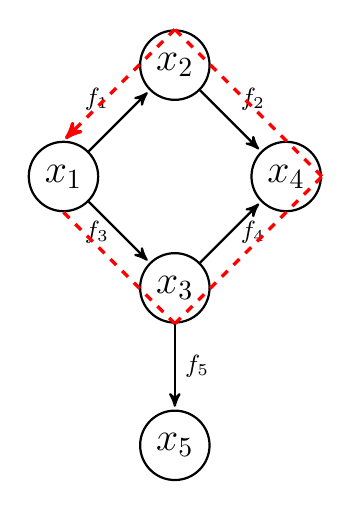
\begin{tikzpicture}[->,>=stealth',shorten >=1pt,auto,node distance=2cm, thick,main node/.style={circle,draw,font=\sffamily\Large\bfseries}]
    \node[main node] (1) {$x_2$};
    \node[main node] (2) [below left of=1] {$x_1$};
    \node[main node] (3) [below right of=2] {$x_3$};
    \node[main node] (4) [below right of=1] {$x_4$};
    \node[main node] (5) [below of=3] {$x_5$};

    \path[every node/.style={font=\sffamily\small}]
        (2) edge node {$f_1$} (1)
        (1) edge node {$f_2$} (4)
        (2) edge node [left] {$f_3$} (3)
        (3) edge node [right] {$f_4$} (4)
        (3) edge node {$f_5$} (5); 

    \draw[dashed,->,color=red,very thick] 
    (2.south) -- (3.south)
    (3.south) -- (4.east)
    (4.east) -- (1.north)
    (1.north) -- (2.north);
    \end{tikzpicture}
    $\mathbf{v_2}$: 
    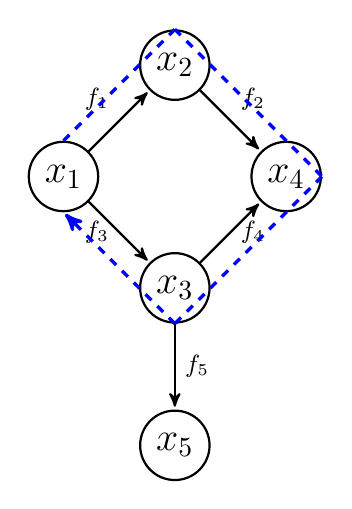
\begin{tikzpicture}[->,>=stealth',shorten >=1pt,auto,node distance=2cm, thick,main node/.style={circle,draw,font=\sffamily\Large\bfseries}]
        \node[main node] (1) {$x_2$};
        \node[main node] (2) [below left of=1] {$x_1$};
        \node[main node] (3) [below right of=2] {$x_3$};
        \node[main node] (4) [below right of=1] {$x_4$};
        \node[main node] (5) [below of=3] {$x_5$};
    
        \path[every node/.style={font=\sffamily\small}]
            (2) edge node {$f_1$} (1)
            (1) edge node {$f_2$} (4)
            (2) edge node [left] {$f_3$} (3)
            (3) edge node [right] {$f_4$} (4)
            (3) edge node {$f_5$} (5); 
    
        \draw[dashed,->,color=blue,very thick] 
        (2.north) -- (1.north)
        (1.north) -- (4.east)
        (4.east) -- (3.south)
        (3.south) -- (2.south);
    \end{tikzpicture}
\end{document}